\chapter*{Introduction}
\addcontentsline{toc}{chapter}{Introduction}
\hypertarget{problem-and-scope}{%
\section{Problem and scope}\label{problem-and-scope}}

An agent has finished a change. The tests pass, and a reviewer is examining a compact diff. The run appears successful, yet the available record may not establish whether another run would produce the same result, whether the tests exercised the relevant behavior, or whether the reviewer saw the decisions that carried the most risk.

The visible output is code; the uncertainty around its quality resides in the system that produced, evaluated, and approved it. A coding agent is one component in that system. Evaluation determines what counts as success, governance constrains access, context management controls the information available during a run, review defines the quality gate, and scheduling allocates compute, money, time, and human attention.

These functions interact. A higher score can result from an easier test rather than a better system. A reviewer can appear ineffective because the interface concealed the evidence needed for judgment. Instrumentation can record component failures while missing failures at component boundaries. A recovery procedure can pass while depending on credentials whose compromise would also destroy the recovery path.

This technical review and engineering monograph examines the evaluation, operation, and governance of AI coding-agent systems. It focuses on mechanisms that remain relevant as models and products change: measurement design, execution-based grading, containment, durable state, recovery, repository retrieval, context limits, human oversight, topology, and resource allocation. It does not compare current models or teach prompt and tool-schema design.

The intended reader is a staff engineer, evaluation lead, or technical owner building a coding-agent evaluation or operations program. The statistical methods are introduced where they affect an engineering decision, but the monograph assumes comfort with experiment design, production controls, and technical review. Its practices are bounded engineering claims rather than universal rules. Their applicability depends on workload, permissions, failure costs, deployment conditions, and available review capacity.

\hypertarget{the-reliability-dependency-chain}{%
\section{The reliability dependency chain}\label{the-reliability-dependency-chain}}

The organizing argument is a dependency chain. Measurement determines whether a difference is credible. Grading converts observations into acceptance decisions. Containment and recovery determine whether the resulting execution record survives failure without extending authority. Retrieval and context determine which evidence reaches the agent. Review and accountability determine who can challenge the result and who controls the consequential transition. Allocation and cost determine which system receives future work.

Each layer determines what the next may trust. A weak measurement can become a confident grade; a weak grade can admit unsafe work; an incomplete recovery record can enter retrieval as if it were complete; missing context can make review appear ineffective; and an invalid review signal can steer more work toward the wrong configuration. Downstream confidence cannot repair evidence lost upstream.

This creates a repair asymmetry. Later machinery is often easier to add than the earlier instrument is to repair, yet it is evaluated through that earlier instrument. More samples cannot repair a task distribution that excludes production work. More judges cannot repair a rubric experts apply inconsistently. More agents cannot repair a retrieval boundary that treats an empty result as authoritative. The dependency chain is therefore a sequence of evidence obligations, not a list of subsystems.

\begin{figure}[htbp]
\centering
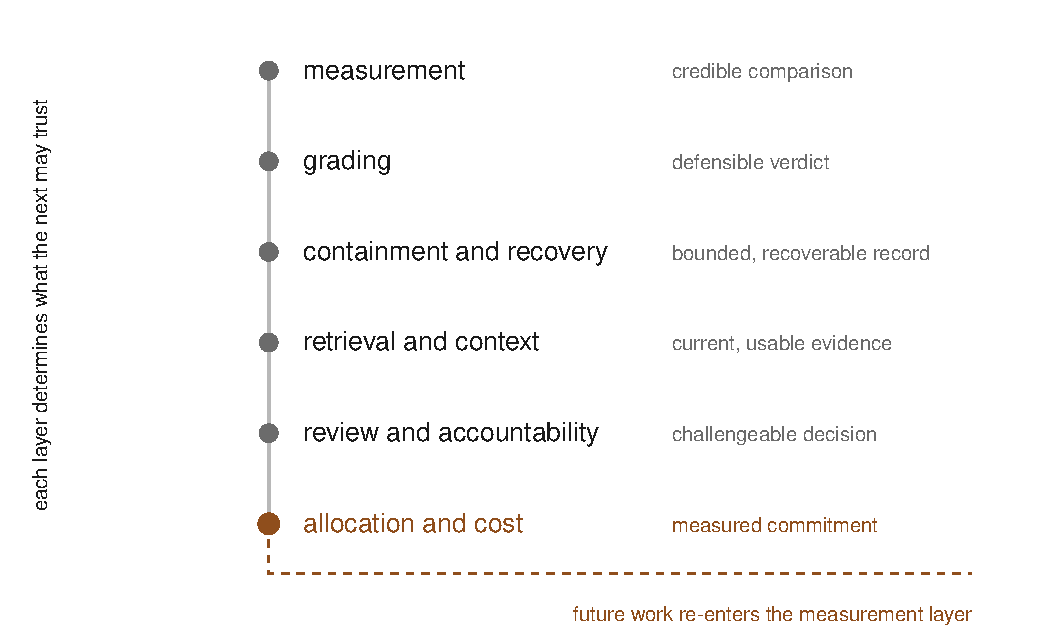
\includegraphics[width=1\textwidth,height=\textheight,keepaspectratio]{figures/dependency-chain.pdf}
\caption{Argument map for the reliability dependency chain: measurement, grading, containment and recovery, retrieval and context, review and accountability, and allocation and cost. Each layer supplies the evidence boundary on which the next relies.}
\end{figure}

The six parts follow this order. It is not a progression from easy to difficult. It is an account of how an apparently local defect can propagate into later operational decisions while retaining the appearance of a clean score, verdict, or artifact.

\hypertarget{method-scope-and-evidence-classification}{%
\section{Method, scope, and evidence classification}\label{method-scope-and-evidence-classification}}

This review treats source collection, evidence grading, practice derivation, and the treatment of author-system cases as separate methodological decisions. The following subsections describe each decision and the limits it places on the resulting claims.

\hypertarget{search-and-source-assembly}{%
\subsection{Search and source assembly}\label{search-and-source-assembly}}

The review was consolidated on July 26, 2026, then subjected to a bounded update audit and a software-engineering venue coverage probe through August 6, 2026. The release-candidate source collection contains 138 scholarly works, 91 practitioner records, 29 benchmark records, and 17 author-system case records. The original 118 scholarly works were organized into seven topic-specific threads covering benchmark validity, failure taxonomy, evaluation statistics, oversight and accountability, context and retrieval, durable execution, and scheduling with repository-scale scoping. Eleven works were admitted during the update audit and nine during the coverage probe.

Scholarly retrieval used \href{https://scixplorer.org/scixabout/}{SciX}, the NASA-supported literature discovery service operated by the Smithsonian Astrophysical Observatory, and a local retrieval layer referred to here as \textbf{SciX Agent}. The official \href{https://scixplorer.org/scixhelp/api-scix/}{SciX API} supplied bibliographic identities and metadata. At consolidation, SciX Agent searched a 32.4-million-record SciX and arXiv corpus with 299.3 million citation links and full text for 14.9 million records. It combined INDUS dense retrieval with BM25 lexical retrieval through reciprocal-rank fusion. These systems determined which records were retrieved and read first; they did not determine evidence grades.

Queries were scoped by topic, subject class, and year where appropriate. Each thread combined seminal work with recent agent-era research. Candidate records were verified by identity, and full text was read when available and when the claim required more than the abstract. A citation audit added the seventh thread after finding scheduling and repository-scoping sources that had entered the draft through adjacent operations-research material.

Practitioner retrieval used the \textbf{\href{https://www.sjarmak.ai/projects/code-intelligence-digest}{Code Intelligence Digest}}, an author-operated corpus that ingests research feeds, engineering publications, newsletters, podcasts, community discussions, and product or operations accounts. At the July 26 cutoff, its local snapshot contained 162,350 normalized records from 149 source labels, including 43,953 records with retained full text. Keyword and semantic retrieval were used within relevant practitioner categories. Research records found through the Digest were moved to the scholarly lane and deduplicated there. Repeated practitioner accounts of one incident shared an independence key and could not be counted as independent corroboration merely because several pages repeated the event.

This practitioner lane makes the review \textbf{multivocal} in the software-engineering sense described by Garousi, Felderer, and Mäntylä (\href{https://doi.org/10.1016/j.infsof.2018.09.006}{2019}): it combines scholarly and grey literature because operational mechanisms and incidents are often documented outside venues. The lane also follows the more restrictive point made by Kitchenham and colleagues (\href{https://doi.org/10.1109/TSE.2022.3165938}{2022}): a mutable social-media post is not treated as a primary study merely because it is informative. Practitioner records remain corroborating cases unless they report a sufficiently specific measurement, and mutable cited pages are archived. The independence key operationalizes source independence by grouping reports that repeat one originating incident or claim.

The benchmark collection was assembled separately from benchmark documentation and publications, merged from two inventories, deduplicated by identity, and validated against a JSON Schema. Three repeated benchmark records were removed during that merge.

The initial scholarly search did not establish adequate coverage of the core software-engineering venue literature. A subsequent OpenAlex metadata probe searched eight topic formulations across ICSE, FSE, ASE, ISSTA, \emph{Empirical Software Engineering}, \emph{IEEE Transactions on Software Engineering}, \emph{ACM Transactions on Software Engineering and Methodology}, and \emph{Computer Supported Cooperative Work}. It surfaced 148 unique candidates. Nine methodologically material works were admitted after title-and-abstract screening, including the SEGRESS reporting guideline (\href{https://doi.org/10.1109/TSE.2022.3174092}{Kitchenham et al.~2022}), the ABC framework for software-engineering research (\href{https://doi.org/10.1145/3241743}{Stol and Fitzgerald 2018}), and work on construct validity in software engineering (\href{https://doi.org/10.1109/TSE.2022.3176725}{Sjøberg and Bergersen 2023}).

That probe diagnosed coverage; it did not replace a publisher-native search. In a deterministic sample of 40 candidate DOIs, SciX contained eight exact DOI matches. The sample is too small and topical to estimate corpus recall, but the missing records are sufficient to reject an assumption of complete SE venue coverage. ACM Digital Library returned HTTP 403 to the automated search client, while the IEEE Xplore and Scopus APIs required credentials not configured in the review environment. The archival first edition is therefore conditional on a supplementary search executed against ACM Digital Library, IEEE Xplore, and Scopus, or on a documented database substitution whose coverage is justified. The companion preserves the probe protocol, all 148 candidates, and the exact SciX comparison.

\begin{figure}[htbp]
\centering
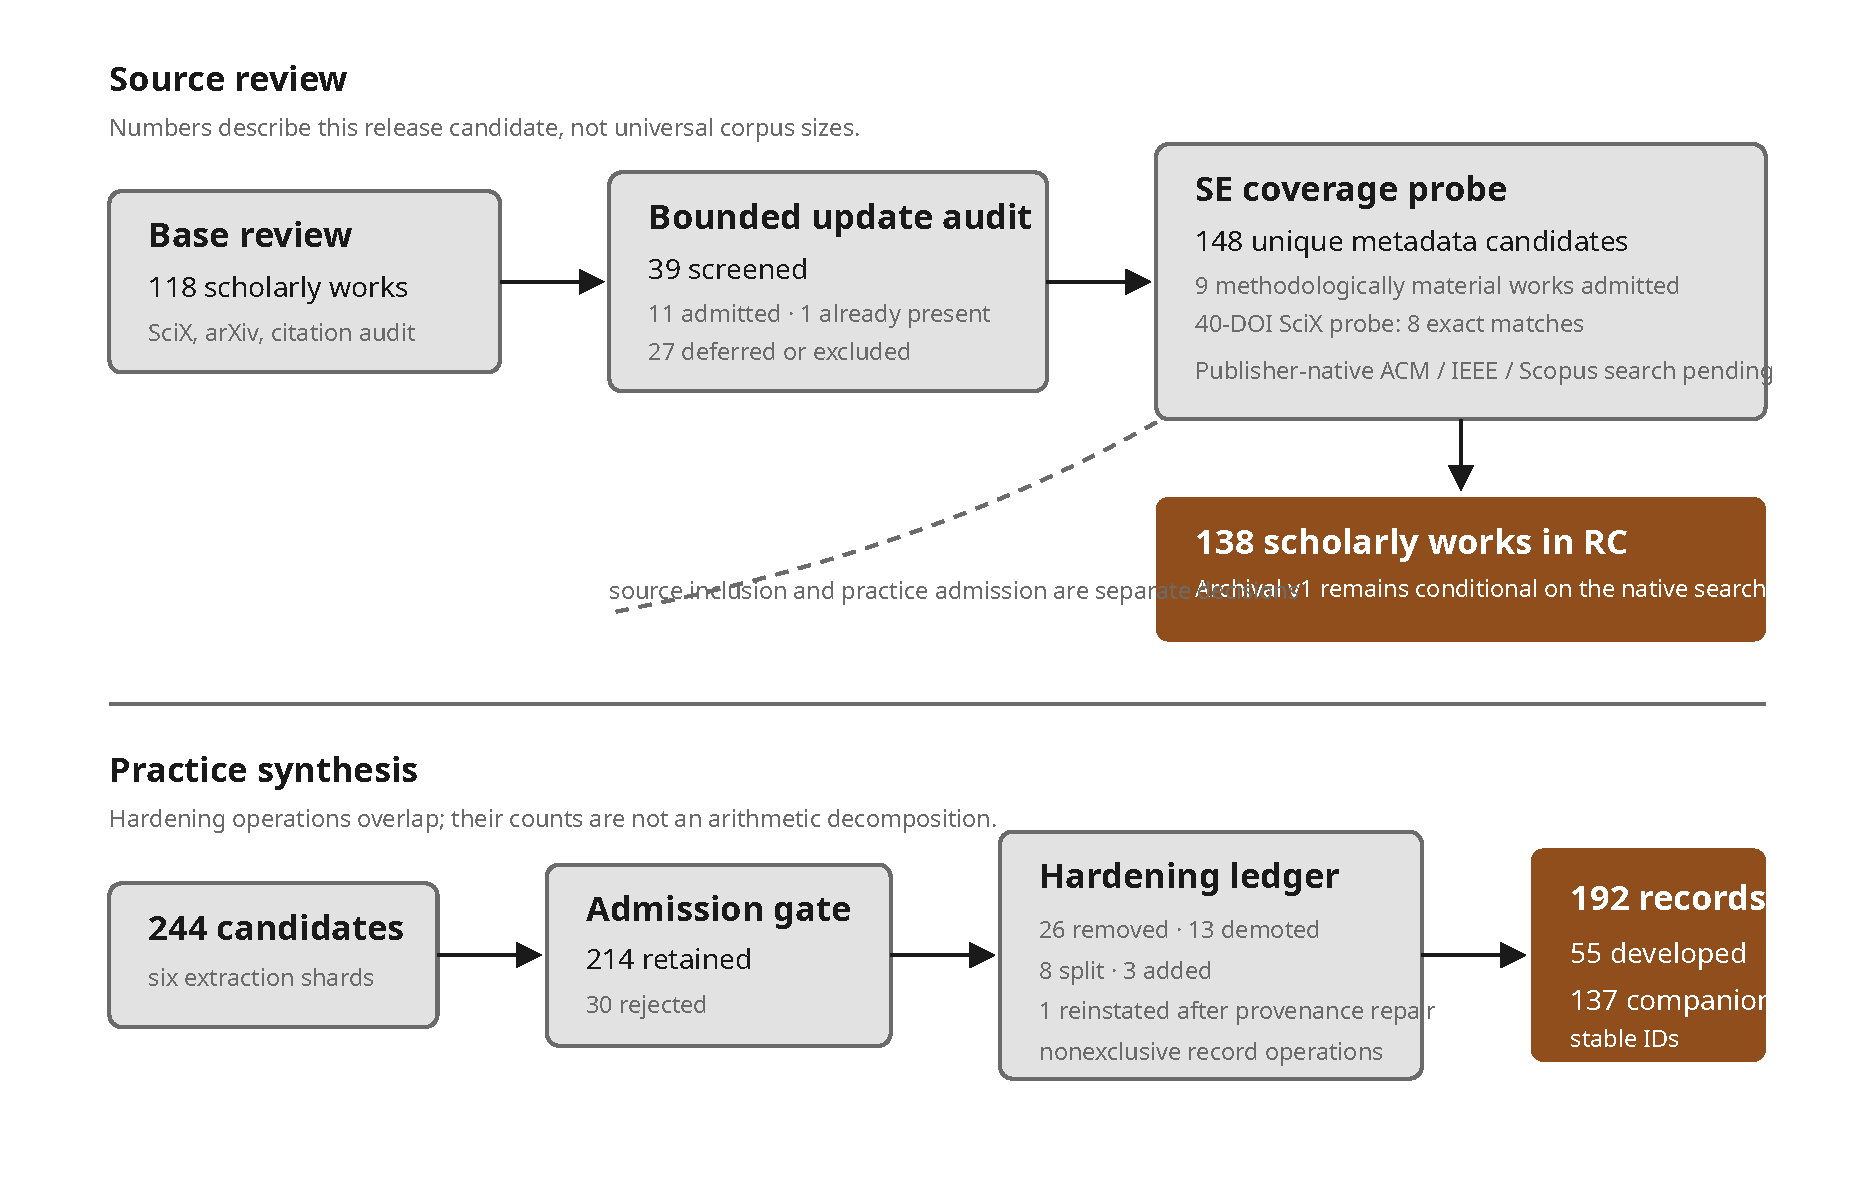
\includegraphics[width=1\textwidth,height=\textheight,keepaspectratio]{figures/review-flow.pdf}
\caption{Flow of source review and practice synthesis. The source lane distinguishes the base review, bounded update audit, SE coverage probe, and the remaining publisher-native search. The practice lane reports the admission gate and overlapping hardening operations without treating their counts as an arithmetic decomposition.}
\end{figure}

The search remains structured rather than exhaustive. It does not cover every scholarly index, venue, private operational record, or adjacent model-comparison literature. The SEGRESS reporting items provide the vocabulary used below: source admission is governed by inclusion and exclusion criteria; evidence-group assignment is a quality assessment of a scoped claim; and practice construction is data extraction and synthesis. These names do not change the underlying decisions, but they make the review easier to compare with software-engineering secondary studies.

\hypertarget{curation-and-assembly-workflow}{%
\subsection{Curation and assembly workflow}\label{curation-and-assembly-workflow}}

The assembly process followed a fixed sequence: define a question for each thread; retrieve candidates; resolve record identity; screen for an in-scope claim; extract the bounded claim and its conditions; assign an evidence group; challenge the assignment; derive candidate practices; select practices for chapter treatment; and audit the final citations. Retrieval rank determined screening order only. A highly ranked record received no evidentiary preference after screening.

Automated systems assisted with retrieval, normalization, duplicate detection, bounded claim extraction, metadata checks, and challenge passes. The cited source remained authoritative. The author made the final decisions about inclusion, evidence grouping, practice admission, chapter placement, and prose. When a challenge pass exposed ambiguity, the lower evidence group was used unless the narrower strong claim could be stated directly.

\begin{longtable}[]{@{}
  >{\raggedright\arraybackslash}p{(\columnwidth - 4\tabcolsep) * \real{0.3333}}
  >{\raggedright\arraybackslash}p{(\columnwidth - 4\tabcolsep) * \real{0.3333}}
  >{\raggedright\arraybackslash}p{(\columnwidth - 4\tabcolsep) * \real{0.3333}}@{}}
\caption{Automation and human judgment in the review workflow. \emph{Automated} means the operation ran without item-level prompting; \emph{assisted} means a system proposed or flagged material for a human decision; \emph{human} means the substantive choice was made without an automated verdict.}\tabularnewline
\toprule\noalign{}
\begin{minipage}[b]{\linewidth}\raggedright
Review step
\end{minipage} & \begin{minipage}[b]{\linewidth}\raggedright
Mode
\end{minipage} & \begin{minipage}[b]{\linewidth}\raggedright
Human decision retained
\end{minipage} \\
\midrule\noalign{}
\endfirsthead
\toprule\noalign{}
\begin{minipage}[b]{\linewidth}\raggedright
Review step
\end{minipage} & \begin{minipage}[b]{\linewidth}\raggedright
Mode
\end{minipage} & \begin{minipage}[b]{\linewidth}\raggedright
Human decision retained
\end{minipage} \\
\midrule\noalign{}
\endhead
\bottomrule\noalign{}
\endlastfoot
Candidate retrieval and ranking & Automated and assisted & I defined each thread question and search boundary, then read the admitted sources. \\
Identity resolution, normalization, and duplicate checks & Automated checks with human resolution & I resolved ambiguous identities and practitioner independence keys. \\
Bounded-claim extraction & Assisted & I checked the source, revised the extracted claim, and accepted or rejected it. \\
Initial evidence-group proposal & Assisted & I assigned the final label to the scoped claim. \\
Challenge pass & Assisted & Automated passes flagged composite claims, contrary findings, duplicate support, and label inconsistencies; I reread the source and adjudicated each change. \\
Practice admission, chapter selection, and prose & Human & I made the selection and writing decisions. \\
Schema, checksum, identifier, and cross-reference gates & Automated verification & A failure blocked the release until the underlying record was corrected. \\
\end{longtable}

The challenge pass was an error-finding aid, not an independent grader. In particular, automated assistance in that pass searched for composite claims, inconsistent evidence groups, contrary findings, duplicate support, and broken identifiers. It did not accept a practice or promote an evidence group.

The update audit screened 38 distinct scholarly records surfaced in Code Intelligence Digest editions published from July 27 through August 5, plus one paper found in a targeted August 6 check. Eleven new works were admitted, one record was already present, and 27 were deferred or excluded. Admission required a material addition to a claim already in scope; novelty or recency alone was insufficient. Material published after August 6 enters the update queue for a later edition unless it corrects a factual error in this one.

Working thread syntheses and source receipts were retained, but the original interactive searches did not preserve every machine-issued query in a publication-ready log. The companion therefore distinguishes retained records from reconstructions. It publishes the source snapshots, sanitized thread protocols, the retained update-search record, and record-level update decisions; it does not present reconstructed query text as an exact historical log. This permits protocol-level review without implying that every interactive search can be replayed byte for byte.

\hypertarget{screening-and-evidence-grading}{%
\subsection{Screening and evidence grading}\label{screening-and-evidence-grading}}

A source entered the working corpus when it contributed at least one measured result, reproducible mechanism, operational incident, benchmark property, or concrete practice relevant to coding-agent reliability. Screening removed records with unresolved identity, no recoverable claim, no relation to a decision in scope, or complete redundancy with a better-supported record. Sources could remain in the review while a proposed practice was rejected; source inclusion and practice admission were separate decisions.

\Needspace{5\baselineskip}

Evidence is reported in four reader-facing groups:

\begin{itemize}
\tightlist
\item
  \textbf{Strong evidence} is an on-claim controlled comparison, validated benchmark result, or comparably specific measurement within stated conditions.
\item
  \textbf{Directional evidence} supports a mechanism, threat model, comparison design, or direction of effect without establishing the complete recommendation, its magnitude, or broad transfer.
\item
  \textbf{Corroborating evidence} consists of case reports, practitioner accounts, or convergent observations that establish plausibility without estimating prevalence.
\item
  \textbf{Null or conflicting evidence} records a result that did not support the expected effect or that materially limits another claim.
\end{itemize}

These labels attach to evidence items and scoped claims, not to publication venues or whole chapters. A composite recommendation does not become strong because several directional sources converge. When no individual controlled study supports the complete recommendation, the text either narrows the claim to the measured component, classifies the transfer as directional, or presents a protocol to test locally. A strong item may therefore support one step of a developed practice while leaving the generalized prescription directional.

The catalog was graded during assembly and then challenged through independent verification passes. A targeted audit examined ten practices whose sole supporting synthesis had been graded strong, together with two restored items. Six grades were reduced because the source demonstrated a hazard, substrate, or adjacent result rather than the stated remedy; six were retained because the controlled comparison matched the claim. Identifier checks, duplicate-identifier gates, thin-evidence rulings, practitioner-independence checks, and contrary evidence were preserved in the audit record. Ambiguous cases defaulted to the lower grade.

The final adjudication was performed by the author. The challenge passes reduced correlated review error, but they do not constitute blinded independent grading by several human reviewers. That creates an asymmetry with Chapter 5, which asks operators to calibrate graders against independent labels before relying on them.

The release artifact therefore includes a deterministic random sample of 20 practices, the associated evidence items with the author's labels hidden, a reviewer response template, and a script that reports pairwise Cohen's kappa, Fleiss's kappa when three readers participate, observed agreement, and disagreement patterns. At least two external readers must complete that pass before archival v1. This release candidate reports no agreement value because no external labels have yet been collected. The author label will be compared after the blinded pass and will not be treated as ground truth. Even after calibration, agreement measures reproducibility of the quality-assessment instrument rather than correctness of every grade.

\hypertarget{practice-derivation-and-chapter-selection}{%
\subsection{Practice derivation and chapter selection}\label{practice-derivation-and-chapter-selection}}

Candidate practices were derived through bounded-claim extraction and synthesis, then passed through a separate admission gate. A record qualified at the final gate through at least one scholarly item, a non-author synthesis with a resolvable scholarly identity, or at least two practitioner items with distinct independence keys. Hardening separated bundled claims, removed redundant or self-defeating records, preserved contrary findings, and repaired provenance. The resulting catalog contains 192 edition records, each with a stable identifier. That total reflects the chosen claim granularity and editorial boundaries; it is not an estimate of how many reliability practices exist. The companion preserves the full record arithmetic and identifies which hardening operations overlap.

Three selection passes ranked the catalog by different criteria: teachability through a bounded case, consequence for an engineering decision, and coverage of the fourteen mechanism clusters. Practices selected by at least two passes formed the base of the developed set. Individual adjudication then repaired thin mechanism coverage and one provenance defect. The resulting 55 practices receive full treatment in the 18 chapters; the remaining 137 appear in the companion catalog.

The consequence ranking also supplies the operational-urgency calculation used later in the monograph. Among its 52 ranked practices, the Spearman correlation between urgency rank and a binary indicator for whether the practice carried at least one strong evidence item was -0.004. The phrase \emph{nearly uncorrelated} refers to this calculation, not to all 192 catalog entries or to a latent universal measure of importance.

The resulting chapter set is an authorial engineering judgment, not an evidence-derived consensus. The near-zero correlation makes that distinction visible. Some practices are included because a controlled comparison measured their effect; others are engineering controls justified by a structural failure mechanism, an observable check, and an asymmetric cost of waiting for trial evidence. Separating a recovery identity from a production identity, for example, can be tested directly against the authority boundary even when no study estimates how often shared credentials cause loss. Imperative section titles name the control or observation to implement; they do not imply a universal effect size or settled prevalence estimate. Where the argument is mechanistic rather than experimental, the chapter supplies a local test and avoids a numerical target.

\hypertarget{author-system-cases-and-limitations}{%
\subsection{Author-system cases and limitations}\label{author-system-cases-and-limitations}}

Cases from systems operated by the author expose mechanisms, original measurements, and reproducible failure cases. They are always treated as illustrations or local measurements. They are not counted as independent external evidence and do not by themselves support a general recommendation.

A \textbf{local artifact} is a record from a system operated by the author and used to expose a mechanism or local measurement. It is not independent external evidence. When its source was uncommitted at the cited revision or its figures were read from source rather than independently remeasured, the chapter states that provenance condition at first use instead of assigning the artifact a second name.

Evidence remains uneven across topics. Several operational questions have only case-level support, recent capability measurements can age quickly, and practitioner reports are vulnerable to selection, survivorship, and reporting bias. The review excludes model-comparison and prompt-engineering literatures except where they bear directly on system reliability. Transfer is especially substantial in Part VI, where observatory scheduling, compute-cluster scheduling, and adjacent multi-agent studies motivate testable designs for coding-agent fleets. That part should be read partly as a research agenda, not as a body of settled deployment guidance.

This section establishes the standard evidence legend for the whole monograph. Later chapters repeat a limitation only when it changes how a particular result may be used.

\hypertarget{contributions}{%
\section{Contributions}\label{contributions}}

\Needspace{5\baselineskip}

This work makes six contributions:

\begin{enumerate}
\def\labelenumi{\arabic{enumi}.}
\tightlist
\item
  a multivocal evidence audit and machine-readable ledger that distinguish direct support, directional findings, corroborating cases, and null or conflicting results;
\item
  a versioned catalog of 192 bounded practice records in this edition, including 55 developed in depth and stable identifiers that connect the manuscript, companion, and implementation artifacts;
\item
  a dependency chain---and its repair asymmetry---connecting measurement, grading, containment and recovery, context management, human oversight, and resource allocation;
\item
  original measurements and failure cases from author-operated systems, explicitly separated from external evidence;
\item
  runnable protocols for local evaluation, capability-boundary testing, recovery testing, trace analysis, and release decisions; and
\item
  five reusable agent skills with practice-level evidence maps, packaged in the project repository as implementation artifacts rather than additional evidence.
\end{enumerate}

The chapters emphasize conditions, measurements, and failure boundaries because an outcome alone rarely identifies why a system succeeded or failed. A useful account traces ownership, permissions, persistence, ordering, and observation while distinguishing correctness from reliability, performance, cost, safety, and usability.

\hypertarget{a-minimum-pass-through-the-dependency-chain}{%
\section{A minimum pass through the dependency chain}\label{a-minimum-pass-through-the-dependency-chain}}

\Needspace{5\baselineskip}

For an existing system, one compact pass produces the minimum record on which later decisions can build:

\begin{enumerate}
\def\labelenumi{\arabic{enumi}.}
\tightlist
\item
  Reopen one decision based on an aggregate score. Run the cheapest credible baseline and the candidate on identical task versions, initially three times per item, and preserve per-item outcomes.
\item
  Record success, reliability, cost, latency, model, harness, prompt, permissions, and pricing snapshot separately.
\item
  Exercise one permitted and one prohibited action with the ordinary identity, including the boundary between primary and recovery resources.
\item
  Verify one recent completion claim from repository or system state and rerun the executable check that makes it true.
\item
  Read twenty failed or unverifiable runs, label the first upstream failure where the trace permits it, and repair the first ordinary causal question the schema cannot answer.
\item
  Before the next promotion run, record the success floor, cost ceiling, task and baseline versions, mechanism condition, and fault-containment guard.
\end{enumerate}

The pass leaves six challengeable artifacts: a paired distribution, a cost-quality record, an observed authority boundary, an independently verified state transition, a seed failure corpus, and a decision rule fixed before the result was known. It is an entry point, not a reliability certificate. The repository artifact \href{https://github.com/sjarmak/engineering-reliable-coding-agents/blob/main/protocols/minimum-reliability-pass.md}{\texttt{protocols/minimum-reliability-pass.md}} supplies the runnable checklist and retained-artifact layout; the chapters develop each step.

\hypertarget{how-the-monograph-is-organized}{%
\section{How the monograph is organized}\label{how-the-monograph-is-organized}}

The monograph has six parts and eighteen chapters. Measurement comes first because every later practice is adopted or rejected through a measured comparison. Nineteen developed practices in Parts II through VI also require a method introduced in Part I. Interleaving those methods with their uses would scatter each method across four or five chapters.

This order places three chapters of experiment design before the agent-specific operating chapters. Later recommendations depend on those definitions and comparison methods.

Part I establishes how I compare systems when runs vary and scores can mislead. Part II turns those measurements into grading and release decisions. Part III addresses containment, persistent state, recovery, and failure analysis. Part IV examines how repository information enters, survives, and leaves an agent run. Part V treats human review as an engineered control with interfaces, escalation rules, and accountable ownership. Part VI is a research agenda for allocating work across agents and models under cost and capacity constraints. Its questions transfer methods from adjacent scheduling and multi-agent literatures rather than presenting settled coding-agent effects.

\begin{longtable}[]{@{}
  >{\raggedright\arraybackslash}p{(\columnwidth - 4\tabcolsep) * \real{0.3000}}
  >{\raggedleft\arraybackslash}p{(\columnwidth - 4\tabcolsep) * \real{0.4000}}
  >{\raggedright\arraybackslash}p{(\columnwidth - 4\tabcolsep) * \real{0.3000}}@{}}
\caption{Parts and chapters in the dependency-chain order.}\tabularnewline
\toprule\noalign{}
\begin{minipage}[b]{\linewidth}\raggedright
Part
\end{minipage} & \begin{minipage}[b]{\linewidth}\raggedleft
Ch
\end{minipage} & \begin{minipage}[b]{\linewidth}\raggedright
Title
\end{minipage} \\
\midrule\noalign{}
\endfirsthead
\toprule\noalign{}
\begin{minipage}[b]{\linewidth}\raggedright
Part
\end{minipage} & \begin{minipage}[b]{\linewidth}\raggedleft
Ch
\end{minipage} & \begin{minipage}[b]{\linewidth}\raggedright
Title
\end{minipage} \\
\midrule\noalign{}
\endhead
\bottomrule\noalign{}
\endlastfoot
\textbf{Part I: Evaluation measurement and experiment design} & 1 & Run-to-run variance, statistical power, and paired comparisons \\
& 2 & Baselines, ablations, and cost-accuracy tradeoffs \\
& 3 & Benchmark contamination, oracle strength, and workload validity \\
\textbf{Part II: Evaluation and grading systems} & 4 & Execution-based evaluation, correction gates, and release tests \\
& 5 & Calibrating model graders and separating agreement from correctness \\
& 6 & Proxy metric gaming and layered evaluation signals \\
\textbf{Part III: Containment, durable execution, and recovery engineering} & 7 & Agent isolation, injection defenses, and independent verification \\
& 8 & Persistent agent state, durable workflows, and idempotent retries \\
& 9 & Replayable traces and fault-injection recovery testing \\
& 10 & Human-auditable failure analysis and taxonomy development \\
\textbf{Part IV: Context engineering: retrieval, budgets, and memory} & 11 & Measuring and designing repository retrieval \\
& 12 & Localization funnels, repository indexes, and freshness checks \\
& 13 & Usable context budgets, consolidated-spec restarts, and file-based tool output \\
& 14 & Cross-session memory, raw traces, and compaction policies \\
\textbf{Part V: Human review and accountability engineering} & 15 & Efficient verification interfaces and risk-based human escalation \\
& 16 & Autonomy calibration, provenance, effective gates, and accountability \\
\textbf{Part VI: Research agenda---work allocation and cost engineering} & 17 & Agent topology selection and dynamic task allocation \\
& 18 & Cost-aware fleet scheduling and model routing \\
\end{longtable}

\hypertarget{what-i-assume-you-know}{%
\section{What I assume you know}\label{what-i-assume-you-know}}

I assume working knowledge of version control, continuous integration, code review, on-call practice, containers, and basic statistics. I use those foundations without rebuilding them. I still describe the relevant system boundary when a familiar tool plays an unfamiliar role.

I assume no prior exposure to the evaluation methods specific to public agent results. I begin with how to read a public score and identify the claim it can support. I then show how many repeated runs a comparison needs before an observed difference carries useful information. The answer depends on variation and the size of the difference you need to detect.

I also teach why agreement with human labels does not by itself make an automated grader correct. Agreement can conceal shared mistakes, ambiguous examples, or a reference answer that measures the wrong property. I separate the observed agreement from the inference made about correctness, which becomes important when a grader controls release.

Another method checks whether a score was earned on work the model had already encountered. I introduce the required vocabulary only when the mechanism appears. My goal is that a technically capable reader should be able to reproduce the reasoning presented in this monograph, not merely accept my interpretation.

The monograph does not assume a particular agent architecture or deployment scale. I describe architecture separately from implementation so the mechanism survives changes in products and interfaces. Examples expose permissions, retries, caching, concurrency, identity, and ordering when those details affect the claim. Code appears only when prose would obscure a state transition or failure path.

\hypertarget{how-to-read-a-chapter}{%
\section{How to read a chapter}\label{how-to-read-a-chapter}}

A chapter opens on a concrete situation, usually a measurement that came out wrong or a failure with a traceable cause. The mechanism follows, then what the evidence does and does not establish, then the boundary conditions, then a procedure you can run. Specialized terms are marked in bold where they are defined, so a term met later can be traced back to that site.

Citations appear inline in author-year form, with the year linked to the source. The back matter of each chapter, headed Sources and evidence, records the evidence grouping, identifier, and claim supported by each item. The back matter is authoritative for identifiers and evidence grouping; the prose states the claim for which a source is used. A disagreement between the two is an editorial defect.

The evidence legend in the methods section applies throughout. Chapter text restates only limitations that materially narrow a particular result, while each unnumbered Sources and evidence section records the claim, identifier, and evidence group for the cited items.

\hypertarget{the-companion-catalog}{%
\section{The companion catalog}\label{the-companion-catalog}}

The \href{https://sjarmak.ai/books/engineering-reliable-coding-agents/companion}{companion site} indexes all 192 practices under the chapter whose mechanism each extends. The 55 developed in the main chapters appear as short pointers into the chapter; the remaining 137 appear as compact entries. The catalog broadens the set of available options without forcing the main text to explain every variation. The \href{https://github.com/sjarmak/engineering-reliable-coding-agents}{project repository} contains the versioned manuscript, evidence ledger, benchmark catalog, schemas, provenance data, and release checksums. The \href{https://sjarmak.ai/books/engineering-reliable-coding-agents}{web edition} provides the browser-oriented reading version.

Use the relevant chapter as the foundation, then consult the catalog for practices that match a specific constraint. A compact entry cannot reproduce the chapter's full treatment of mechanism, evidence, tradeoffs, and failure boundaries. The chapter provides the reasoning needed to decide whether a neighboring practice applies to your workload.

Twenty-nine of the full entries are labeled as limited-support notes. I excluded them from the developed set because the available evidence does not support a recommendation. Treat them as prompts for investigation rather than established guidance. They may point to a useful experiment, a missing control, or a failure mode worth instrumenting.

The chapters and catalog serve different purposes. The chapters develop methods and claims in enough detail to evaluate critically. The catalog preserves breadth and makes related practices easier to find. Together, they let you begin with a measured problem and identify an intervention suited to the system you actually operate.

The repository also packages five reusable agent skills derived from selected practices: evaluation design, end-to-end test design, failure-mode capture, focused execution, and verified long-running implementation. Each skill includes a practice-level evidence map. These are implementation artifacts intended to make the protocols reusable; they are not additional evidence that the practices work across environments.

This edition is versioned because capability measurements and source availability change. The evidence ledger is scheduled for an annual review, with an out-of-cycle release when a material factual error, citation failure, or retraction changes a claim. Stable practice IDs persist across those releases; a later edition may retire, split, or merge a record without silently reusing its identifier.

\hypertarget{what-you-should-be-able-to-do-by-the-end}{%
\section{What you should be able to do by the end}\label{what-you-should-be-able-to-do-by-the-end}}

Given a published agent score, you should be able to state the narrower claim it supports and identify the conditions on which that claim depends. Given a proposed change to your own system, you should be able to measure run-to-run variation before crediting a difference and size the comparison before spending the model calls. Both systems should run on the same items, and a design that cannot resolve the difference relevant to the decision should return no verdict. Cost belongs in that judgment alongside accuracy, as does the possibility that a simpler configuration would have performed just as well.

You should be able to assess whether a public score was earned on tasks the model may already have encountered and to build an evaluation set from your own repositories when the public benchmark does not represent your work. Grades should rest on execution rather than the model's confidence, and automated graders should be validated against human labels before they gate releases. When a proxy improves without a corresponding improvement in the outcome it represents, the system should make that divergence visible.

Operationally, you should be able to bound what a single run can access and destroy, and you should treat an agent's account of its own work as a claim that still requires verification. A run that fails partway through should leave a durable record of which steps completed, and every retried step should be safe to execute again. Recovery should be tested by injecting failures rather than inferred from an architecture diagram. Reading a hundred traces from your own system should yield a concrete failure taxonomy.

Retrieval should be evaluated separately from generation so that a wrong answer can be attributed to the stage that produced it. You should also be able to measure how much of an advertised context window the system can use effectively. Human review should occur where the reviewer can see the decision that carries the risk, and autonomy should expand by action type only when measured approval and modification rates justify it. A multi-agent design should be required to outperform a single agent on the same tasks, and each component should run on the least expensive model that can perform its role reliably.

The goal is to provide you with the tools to measure what matters for your work, so the result describes the system you operate rather than a position on a leaderboard.
